\documentclass[12pt]{article}

\usepackage[slovak]{babel}
\usepackage[utf8]{inputenc}
% \usepackage[cp1250]{inputenc}
\usepackage[T1]{fontenc}
\usepackage{latexsym}
\usepackage{graphicx}
\usepackage[section]{placeins}

\title{Zadanie 2: Komunikácia s využítím UDP protokolu}
\author{
        Počítačové a komunikačné siete\\
        \\
        Ema Richnáková \\
        Piatok 08:00 \\
        FIIT STU\\
}
\date{\today}

\begin{document}
\clearpage\maketitle
\thispagestyle{empty}

\pagebreak
\setcounter{page}{1}

\section{Úloha zadania}\label{task description}
Navrhnite a implementujte program s použitím vlastného protokolu nad protokolom
UDP (User Datagram Protocol) transportnej vrstvy sieťového modelu TCP/IP. Program umožní
komunikáciu dvoch účastníkov v lokálnej sieti Ethernet, teda prenos textových správ a
ľubovoľného súboru medzi počítačmi (uzlami).

Program bude pozostávať z dvoch častí – vysielacej a prijímacej. Vysielací uzol pošle
súbor inému uzlu v sieti. Predpokladá sa, že v sieti dochádza k stratám dát. Ak je posielaný
súbor väčší, ako používateľom definovaná max. veľkosť fragmentu, vysielajúca strana rozloží
súbor na menšie časti - fragmenty, ktoré pošle samostatne. Maximálnu veľkosť fragmentu
musí mať používateľ možnosť nastaviť takú, aby neboli znova fragmentované na linkovej
vrstve.

Ak je súbor poslaný ako postupnosť fragmentov, cieľový uzol vypíše správu o prijatí
fragmentu s jeho poradím a či bol prenesený bez chýb. Po prijatí celého súboru na cieľovom
uzle tento zobrazí správu o jeho prijatí a absolútnu cestu, kam bol prijatý súbor uložený.
Program musí obsahovať kontrolu chýb pri komunikácii a znovuvyžiadanie chybných
fragmentov, vrátane pozitívneho aj negatívneho potvrdenia. Po prenesení prvého súboru pri
nečinnosti komunikátor automaticky odošle paket pre udržanie spojenia každých 10-60s pokiaľ
používateľ neukončí spojenie. Odporúčame riešiť cez vlastne definované signalizačné správy.


\section{Analýza protokolov UDP a TCP}\label{UDP TCP analyze}
\subsubsection*{Spoločné vlastnosti}
Oba protokoly sú určené na prenos dát po internete, ktoré rozdeľujú do tzv. paketov (balíčkov). 
Oba pracujú nad \textit{Internet protokolom} (ozn. IP).

\subsubsection*{Rozdielne vlastnosti}
Hlavný rozdiel medzi nimi je ich účel využitia.
\begin{center}
        \begin{tabular}{ | p{3cm} | p{5cm} | p{5cm} | }
        \hline
         & TCP & UDP \\ \hline

        Spoľahlivosť & 
        Spoľahlivý protokol, ktorý garantuje spoľahlivosť dátového prenosu vďaka dôkladnejšej 
        kontrole rozkúskovaných dát pri komunikácii medzi zariadeniami. & 
        Nespoľahlivý protokol, ktorý uprednostňuje rýchlosť prenosu, a teda jeho kontrolné 
        algoritmy sú jednoduchšie, čo môže spôsobiť neúplnosť prenesených údajov. \\ \hline

        Kontrola chýb & 
        Rozšírený mechanizmus kontroly. Ponúka tzv. flow control (kontola toku dát). & 
        Základná kontrola (checksum). \\ \hline

        Poradie paketov & 
        Sekvencia dát sa zachová. & 
        Sekvencia dát sa nemusí zachovať. \\ \hline

        Rýchlosť & 
        Pomalší protokol, kvôli zabezpečeniu spoľahlivosti dátového prenosu cez nespoľahlivé 
        siete. & 
        Rýchlejší protokol, pre malý objem réžijných dát a jednoduchej kontrole pri prenose. 
        \\ \hline

        Strata paketov & 
        Ak takáto situácia nastane, stratený paket zaradí na jeho správne miesto ešte pri 
        prenose. & 
        Stratený paket nenájde. Prijímacie zariadenie si ho musí znovu vypýtať. \\ \hline

        Hlavička (max. veľkosť) & 
        20-80 B & 
        8 B \\ \hline
        \end{tabular}
\end{center}


\newpage

\section{Návrh programu}\label{program}
\begin{figure}[h!]
        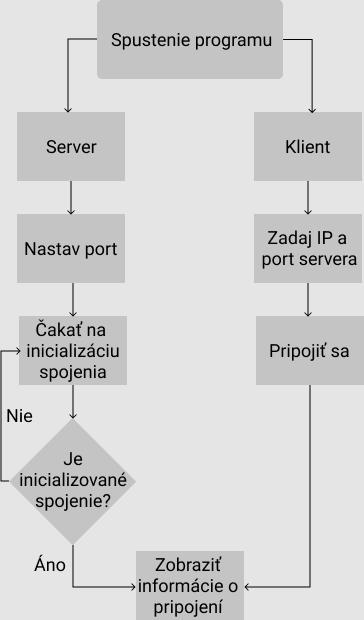
\includegraphics[width=0.5\linewidth]{images/connection-init.png}
        \caption{Inicializácia spojenia}
        \label{fig:classDiagram}
\end{figure}

\section{Interakcia používateľa s projektom}\label{conclusions}
Používateľovi sa po načítaní aplikácie ukáže menu, v ktorom vie vybrať možnosť 
\textit{Spustiť hru}. Po spustení sa scéna presunie na bojisko. Konkrétne sa bude nachádzať 
na hradnom opevnení. Pohľad bude z pvej osoby, čiže bude vedieť manipulovať s kamerou. 
Taktiež sa na opevnení bude nachádzať aspoň jedna zbraň, ku ktorej sa používateľ vie 
premiestniť a vie ju tlačidlom použiť a strielať z nej. Pri streľbe sa na obrazovke v strede 
zobrazí mieridlo, ktoré pomôže používateľovi lepšie mieriť na nepriateľa.

\section{Pseudokódy}\label{pseudocodes}
Použitie zbrane používateľom:
\begin{verbatim}
        Ak hráč koliduje s objektom zbrane 
        a ak stlačí tlačidlo Medzerník 
        prepne sa kamera na pohľad zbrane - začne ju ovládať 
        ľavým tlačidlom myši používateľ strieľa a myšou ovláda kameru
        znovu stlačenie medzerníku používateľ zruší používanie zbrane
\end{verbatim}
Útok nepriateľa na hrad:
\begin{verbatim}
        Ak nepriateľ pretne hranu obrazovky
        zníži sa počet životov hradu o toľko 
        koľko poškodenia dáva nepriateľ
\end{verbatim}
Zničenie nepriateľa:
\begin{verbatim}
        Ak projektil koliduje s nepriateľom
        a je to slabý nepriateľ
        nepriateľa zničí
        inak ak je to silný nepriateľ
        uberie mu polovicu života
\end{verbatim}

\section{Metódy renderovania štruktúr na obrazovku}\label{rendering}
Renderovanie bude prebiehať v reálnom čase, kedže scéna bude interaktívna, prvky budú 
manipulovatelné a dynamické (napríklad nepriatelia, ktorí po zničení zmiznú). Na 
osvetlenie/reflekciu svetla sa bude používať Phongov algoritmus. Na tieňovanie bude použití 
bump mapping.

\section{Zapojenie jednotlivých komponentov aplikácie do funkčného celku}\label{functioning unit}
Obloha tvorí pozadie scény a zároveň vytvára obmedzený priestor, kde sa môžu nepriateľské 
jednotky pohybovať. V strede tejto scény sa nachádza hrad na vznášajúcom sa ostrove. Okolo 
neho poletujú určenými smermi nepriateľské letecké jednotky. Používateľ sa nachádza na hradnom 
opevnení spolu so zbraňami. Používateľ vidí svet z prvej osoby, čiže priamo ovplyvňuje 
sklon, smer a pohyb kamery. Používateľ sa vie pohybovať v obmedzenom priestore hradného 
opevnenia. Vie interagovať so zbraňami na opevnení tak, že preberie nad nimi kontrolu a 
vie nimi odstrelovať nepriateľov. Projektil zbrane po kolízií s nepriateľom uberie nepriateľovi 
životy. Používateľ taktiež vie odísť od zbrane a znovu sa vie 
pohybovať po opevnení. Hlavné osvetlenie bude tvoriť slnko. Druhý zdroj osvetlenia budú 
fakle pripevnené na vnútorné steny opevnenia. Oheň by mal taktiež reagovať na vietor a 
teda mal by sa podľa jeho smeru naklánať. Vietor by taktiež mohol ovplyvňovať trajektóriu 
projektilu zbrane.

\end{document}